% このファイルの文字コードは UTF-8
% 環境はtexlive2018
%\documentclass[11pt, a4paper]{ujreport} %イキッてuplatexを使っているだけなので
\documentclass[11pt, a4paper]{jreport} %普通にplatexのこっちでいいと思われる(違いが知りたければggってください)
\usepackage[dvipdfmx]{graphicx} %画像読み込み用 texの壁なのでggって,どうぞ
\usepackage{thesis} % ここで表紙のテンプレ他を作ってる
\usepackage{url}
\usepackage{ascmac}
\usepackage{algorithm,algorithmic}
\usepackage{booktabs}
\usepackage{comment}
\usepackage{here} %個人的に必須だと思っている.これがあると画像表示のとき[H]が使えるようになる.(その場所に画像を置く)
% 参考文献のとこで使う
\renewcommand{\bibname}{参考文献}


%タイトル
\title{タイトル}
\author{名前}
\date{平成〇年〇月〇日} 

\begin{document}
\maketitle

%概要
\begin{abstract}
概要
\end{abstract}

%目次
\tableofcontents
% 本文

%%%%%%%%%%%%%%%%%%%%%%%%%%%%%%%%%%%%%%%%%%%%%%%%%%%%%%%%%%%%%%%%%
% 1章 序論
%%%%%%%%%%%%%%%%%%%%%%%%%%%%%%%%%%%%%%%%%%%%%%%%%%%%%%%%%%%%%%%%%
\chapter{序論}

序論

\chapter{本研究の背景と目的}


\section{哲学対話}
\subsection{哲学対話の目的}

\subsection{哲学対話に必要な支援}
% まずは参加すること。それが探求の共同体へつながっていく様子みたいな図

\section{関連研究}
% ~じゃだめで~ 今までにない支援方法が必要

\section{本研究の目的}
\label{sec:目的}
% どこを支援するのかを絞って書く

\section{本稿の構成}
% 作ってる途中で、いろいろ実験してまっせ



\chapter{議論支援システムの開発と評価実験1}
% 議論システムのプロトタイプを作って実験した 目的はこれこれの知見を得ること。確認したかったのは以下の二点つらつら

本章では、%どうするよ?
哲学対話を支援することを目的とした、ロボットが介在する選択式議論システム(Robot Mediated Selection Based Discussion System: RMSBD)のプロトタイプの開発と評価実験について報告する。\ref{sec:要件1}では設計指針を\ref{sec:目的}で行った目標設定に対応させて整理し、\ref{sec:構成1}で実装したシステムの構成を記す。\ref{sec:実験1}で評価実験について報告する。




\section{システムの設計}
\label{sec:要件1}
% とぴっくごとにする、選択肢をつくる、云々



\section{システムの構成}
\label{sec:構成1}
実装した議論システム(以下、RMSBD-1と呼称する)は、(a)発話データベース、(b)中央処理部、(c)ユーザインターフェース、(d)発話ロボットからなる。以下に、それぞれの部分の詳細と全体の概略を示す。

\subsection*{(a)発話データベース}
\subsubsection*{意見データベース}
\ref{sec:目的}で述べたように、議論中にユーザに提示する選択肢は議題ごとに事前に用意した。発話候補は以下のような手続きで収集、編集を行った。
\begin{enumerate}
\item Google Formを利用した意見の収集\\
オンラインで募集した研究協力者に、議題に関連する複数の意見に対する賛否と、その理由を答えさせた。以下に、論題「愛とは何か」の発話データベースを構築するために作成した質問を例示する。
\begin{quote}
これからいくつかの意見を提示させていただきます。それに賛成か、反対かを回答した後、その回答の理由を別の角度から二つ記述してください。
\begin{itemize}
\item 「お金は愛よりも大切である」という意見に対して
\begin{itemize}
\item 上記の意見に賛成か反対かを教えて下さい。
\item それはなぜですか?「〜から」で終わる一文で答えてください。かならず「〜から」もご自身で記入してください。
\item それはなぜですか?異なる観点からもう一つ理由を答えてください。「〜から」で終わる一文で答えてください。かならず「〜から」もご自身で記入してください。
\end{itemize}

\item 「愛は人の判断を誤らせる」という意見に対して
\begin{itemize}
\item 上記の意見に賛成か反対かを教えて下さい。
\item それはなぜですか?「〜から」で終わる一文で答えてください。かならず「〜から」もご自身で記入してください。
\item それはなぜですか?異なる観点からもう一つ理由を答えてください。「〜から」で終わる一文で答えてください。かならず「〜から」もご自身で記入してください。
\end{itemize}
\end{itemize}
\end{quote}

\item 収集した意見からの論点抽出\\
上記のGoogle Formの回答のうち、それぞれの質問に対する賛否の理由の記述を整理し、論点の抽出を行った。
論点の抽出にあたって、まずそれぞれの記述の前提となっていると考えられる信念をいくつかの類型に分類した。その後、分類をもとに論点を構成した。この作業はシステムの設計者である筆者が行った。
以下に、この作業の進行過程の例を示す。
\begin{quote}
「お金は愛よりも大切である」という意見に賛成する理由として、以下のような記述が得られた。
\begin{itemize}
\item \textsl{お金があるのは手段でしかなく、愛は目的になりうるから。}
\item お金は二次報酬だから。
\end{itemize}
また、反対の理由として、以下のような記述が得られた
\begin{itemize}
\item 費用対効果の面から愛はある一定値に収束する一方、お金は単調増加で豊かになるから。
\item (取引されるサービスやものに対する)愛の度合いを相対的に示す数値がお金だから
\end{itemize}


以上のような記述の背景には、「愛とは○○のようなものである。それに対し、お金とは△△ようなものである」といった信念が存在すると考えられる。以上を踏まえ、「愛とお金はどう違うのか」という論点を形成した。
\end{quote}

% 論点の抽出はシステム設計者が行った。
% 基準を書いて例も載せる
\item  論点の構造化と発話候補の割り当て\\
前述の要領で抽出された論点を階層的に整理した。以下の手順によって構造化を行った。
\begin{enumerate}
\renewcommand{\labelenumii}{(\arabic{enumii}).}
\item それぞれの論点に対し、最も関連すると思われる他の論点を選び、二論点間にリンクを張る。
\item リンクが多く、さらにある程度抽象的だと考えられる論点を、最上位論点として、3個設定する。
\item 1で張ったリンクのうち、最上位論点以外の論点に対し、最上位論点から最短経路で辿るときに経由するもの以外を削除する
\end{enumerate}


次に、構造化された論点に対し、前述の方法で収集された意見を割り振った。この際、同一内容と思われるもの、単体の発言としては理解が困難と考えられるものを省いて割り振った。また、論点に対する意見が十分な数ではない場合には、個別の論点に対する意見を数人の研究協力者に記述させ、発話候補を確保した。



また、意見収集時に同じ質問に対して賛成の立場から記述された意見と、反対の立場から記述された意見は、矛盾する意見としてラベリングした。%この作業により、ある発話候補$u$に対し、その発話と矛盾する発話候補の集合が確定する。


最後に、論点ごとに、別の論点からその論点に遷移させる際に発せられる発話を割り当てた。例えば、「愛とお金はどう違うのか」という論点に対しては、「愛とお金はどう違うのかな?」という発話を、また「愛によって人はどう変わるか」という論点に対しては、「愛によって人はどう変わると思う?」という発話を割り当てた。


以上の作業をまとめると[図]のようになる。
% 木構造にしたものの図を張り付ける

図
図
図
図


これらの作業は、質問や論点に対する意見の記述を除き、システムの設計者である筆者が行った。以上の作業により、テーマに対する様々な意見を整理したデータベースを作成した。
\end{enumerate}
\subsubsection*{その他の発話}
RMSBD-1は、構造化された発話データベースの他に、あいづち、接続語、ファシリテーション発話のデータベースを持つ。
%あいづちは、間接的に意見を主張するのに用いることができる。ファシリテーション発話は、議論の進行を円滑化

\begin{itemize}
\item あいづち\\
前の発話に対してあいづちを打つことで、間接的に意見を主張できると考えられる。本システムでは、以下のあいづちを発話データベースに登録した。
\begin{itemize}
\item 同意、共感を表すあいづち\\
「やっぱそうだよね」、「たしかに」、「わかるわかる」、「そのとおりだよ」、「わかる気がする」
\item 非同意、反論をあらわすあいづち\\
「それは違うと思う」、「うーん」、「そうなのかな」、「えー」、「それには反対だな」
\item 傾聴を表すあいづち\\
「なるほど」、「うんうん」

\end{itemize}

\item 接続語\\
接続語を意見の前に付けて発話することで、発言が持つニュアンスや前の発言に対する関係を明示的にすることができる。本システムでは、以下の接続語を発話データベースに登録した。
\begin{itemize}
\item 順接\\
「じゃあ」、「だから」、「たしかに」、「そして」
\item 逆説\\
「だとしても」、「でも」、「だけど」、「とはいえ」
\item 並列\\
「なおかつ」、「それから」、「しかも」、「その上」、「さらに」
\item 対置\\
「反対に」、「むしろ」、「逆に」、「一方で」
\item 転換\\
「それじゃあ」、「ところで」、「話は変わるけど」、「そういえば」、「じゃあさ」
\end{itemize}

\item ファシリテーション発話\\
ファシリテーション発話は、議論の進行を円滑化させる働きを持つと考えられる。本システムでは、以下のファシリテーション発話を発話データベースに登録した。
\begin{itemize}
\item 議論の流れに言及する発話\\
「ちょっと込み入ってきたし、違う視点から考えられないかな」、「なにか質問の仕方を変えてみるのはどうかな」
\item 議論の現状を確認する発話\\
「難しくなってきたね」、「こうしてみるといろいろな意見があるね」
\end{itemize}

\end{itemize}




\subsection*{(b)中央処理部}
中央処理部は「1. 論点遷移の管理と発話選択肢の抽出」、「2. ユーザインタフェースとの通信」、「3. ロボットとの通信」という三つの処理を行う。

%以下の説明のために、ユーザインタフェースとロボットを以下のように表示する。


今後の説明では、変数は以下の表記を用いる。
議論に参加するユーザ数を$N$とする。
接続されたユーザインタフェース端末を$T_n (n = 1, 2, \dots, N)$とする。接続されたロボットを$R_n (n = 1, 2, \dots, N)$とする。ここで、ユーザインタフェース端末とロボットの添え字の番号はユーザ番号を表し、それぞれの数字は同じユーザに対応しているものとする。


\subsubsection{1. 論点遷移の管理と発話選択肢の抽出}
各インターフェース端末上に表示させる発話候補は、以下のアルゴリズムによって決定される。


「(a)発話データベース」に記した方法により構成した発話データベース上では、各論点$A_x$は、親論点$A_{parent}$と、子論点の集合$A_{child}$を持つ。ただし、末端の論点の場合には子論点の集合は空集合である。ある論点$A_x$に割り当てられた意見の集合を$Op(A_x)$とする。他の論点からある論点$A_y$に移動する際に発せられる発話を$u_{transition}(A_y)$とする。
また、以下の記述では、ある論点上で発話が行われた回数をターン数$t$とする。


ユーザ$p_i$がそれまでに行った発話の集合を$U(p_i)$とする。また、各発話$v \in U(p)$に対し、$v$と矛盾する発話の集合を$Op_{contradict}(v)$とし、各ユーザの過去の発話のどれかに矛盾する発話の集合を$Op_{contradict}(p_i)$とする。各ユーザの過去の発話のどれとも矛盾しない発話の集合を$Op_{concrete}(p_i)$とする。また、議論が発展する速さをコントロールする定数として、$pace$が与えられているものとする。この定数は、一つの論点にとどまり続ける最低ターン数を表す。


現在、議論が論点$A_i$にあるとする。ターン数が$t$であるとする。
\begin{algorithm}
\caption{発話選択肢の抽出}
\begin{algorithmic}[1]
\IF{$t < min(pace, |Op(A_i)|$}%まだ十分にターンが経っていない  %このifのそとには、なにも選ぶものがなかった時の選び方もある
 \STATE $x <= pop(Op(A_i) \cup Op_{concrete}(p_i))$
 \STATE $return x$
 \IF {$aa$}
 \STATE aa
 \ENDIF
\ELSE
 \STATE aa
\ENDIF

\end{algorithmic} 
\end{algorithm}





\subsubsection{2. ユーザインタフェースとの通信}
抽出された発話は、TCPソケットを通じてユーザインタフェースに送信される。
%ユーザインタフェース上で選択された発話接続されたロボットに対して命令を送信する(以下の「3. ロボットとの通信」を参照)。
また、あるユーザインタフェースから発話を受信した際には、その発話をロボットが行うのに要している時間中は全ての端末上での操作を禁止する。

%他の人が発話中はブロック

\subsubsection{3. ロボットとの通信}
ユーザインタフェースから発話の指令を受け取ると、ロボットに対して操作命令を送信する。以下に、命令を生成する規則を説明する。
\begin{itembox}[l]{ロボットに対する操作命令の送信}
$T_i$から発話を受信したとする。この時、中央処理部は$R_j (j \neq i)$に対し、$R_i$が設置された方向を向くように命令を送る。また、$R_j$には発話を行うように命令を送り、同時に発話に合わせたジェスチャーを行わせるように命令を送る。%この時、pythonライブラリであるpykakasiを用いて、発話内容をひらがな化し、ひらがな化された発話の文字数から発話時間を見積もった。
\end{itembox}
%発話の選択肢 選んだらロボットがそっちを向く
% 木を探索する様子、

\subsubsection*{実装環境}
中央処理部の実装にはpythonを用いた。


\subsection*{(c)ユーザインタフェース}
ユーザインタフェース上には、「1. 発話選択肢」と「2. 選択肢更新ボタン」が表示される。
\subsubsection*{1. 発話選択肢}
ユーザインタフェースには、中央処理部から送信された発話の選択肢が表示される。[図]に示すように、最上段には接続語の選択肢が3つ表示される。二段目には意見データベースから抽出された発話が表示される。三段目には、同意、共感を表すあいづちまたは傾聴を表すあいづちが表示される。四段目には、非同意、反論を表すあいづちが表示される。

図
図
図
図


接続語を選択してから意見またはあいづちを選択することで、接続語を意見やあいづちの前に発話させることができる。接続語を選択せずに意見またはあいづちを発話することもできる。

\subsubsection*{2. 選択肢更新ボタン}
インタフェース上には「他の発話」というボタンを設置した。このボタン押すと、選択肢を更新する要求が中央処理部に送られる。その後、インタフェース上に表示される選択肢が別のものに更新される。
%には別の発話の選択肢が表示される。

\subsubsection*{実装環境}
ユーザインタフェースの実装にはpythonを用いた。また、ユーザインタフェース用のプログラムをMicrosoft Surface上で実行し、タッチスクリーン上で選択肢を選ぶことができるようにした。%上述のように(「\textbf{(b)中央処理部}」を参照)、選択された発話は中央処理部を介して発話ロボットに送られる。

\subsection*{(d)発話ロボット}
ユーザインタフェース上で選択された発話は、ロボットに読み上げられる。本システムでは、Vstone社製のCommU\footnote{\url{https://www.vstone.co.jp/products/commu/index.html}}を使用した[図]。CommUは、全身14自由度を持ち、発話と同時に、表情やジェスチャーの表出を行うことができる。発話を行う際には、胸部のスピーカから音声を流しつつ口部関節を振動させることで、実際に話しているような印象を与える。


図
図
図
図


本システムにおいて、CommUはユーザインタフェース上で選択された発話に連動し、「発話時のジェスチャー」、「発話しているロボットの方向の注視」という二種類の動作を行う。これらは、中央処理部からの操作命令に従って行われる(命令の送信については「\textbf{(c)ユーザインタフェース}」の項を参照)。


\subsection{システム動作のフローチャート}
以上にまとめた議論システムRMSBD-1の動作を、[図]のフローチャートに示した。


\section{評価実験}
\label{sec:実験1}
%哲学的の定義が上でなされているはず
評価実験では、開発した議論システムを用いて行う議論で、口頭で行う議論と同程度の参加感および満足感が得られるかを検証した。
開発した議論システムを用いた議論では、参加者は自ら発話内容を考えて口頭で発話するのではなく、選択肢を選びロボットに発話させることで参加する。この設計によって、自ら発話内容を考えること、また考えた内容を発話することが難しい議論への参入障壁を下げることを意図している。


一方で、このシステムを用いた議論では、発話内容や進行に制約があるため、参加感や満足感が口頭で行う通常の議論よりも低いものになる可能性がある。
システムを用いた議論が、参加が難しい人にとって、議論への導入として十分に機能するためには、
議論への参加が難しいかに関わらず、
口頭で行う通常の議論と同程度の参加感や満足感をもたらすものである必要があると考えた。

そこで、大学生の参加者を集め、実験室実験で評価を行った。

\subsection{実験課題}
テーマを「愛」および「働くこと」とし、15分間でテーマについての共通理解を得られるように議論することを課題とした。


\subsection{実験参加者}
大学生24名(男性12名、女性12名、平均年齢XX歳($SD=XX$))が3名1組で実験に参加した。それぞれのグループは全員初対面の同性であった。

\subsection{実験条件}
実験条件は、システムあり条件とシステムなし条件の2条件の被験者間計画であった。
システムあり条件では、議論システムを用いた議論を15分間行った後、中断を挟み、続きの議論をシステムを用いずに15分間行った。
システムなし条件では、議論システムを用いない議論を15分間行った後、中断を挟み、続きの議論をシステムを用いずに15分間行った。
テーマは全グループの半分が「愛」を、半分が「働くこと」を与えられた。2回の議論では、同じテーマについて議論させた。


2回議論を行わせたのは、システムあり条件での議論が、後の議論に与える影響を予備的に観察するためである。1回目の議論の後に記入させた質問紙から得られたもののみを分析の対象とした。

\subsection{事前準備}
実験のため、事前に「愛」および「働くこと」について、\ref{sec:構成1}で示した手順に従って構造化された発話データベースを作成した。また、操作説明のために「日本食」についての発話データべースを作成した。「日本食」を題材として議論システムの使用方法を説明することは、「愛」および「働くこと」についての議論に影響を及ぼすことはないものと考えた。

\subsection{実験手続き}
%appendixとかにつけとくべき
実験参加者から、実験室に入室する前に、書面によるインフォームドコンセントをえた。実験参加者は、実験室に到着次第待合室で「実験では2回議論を行う」旨を伝えた。また、テーマの提示もここで行った。さらに、「行う議論は哲学的なものである」旨を伝え、「話している人を遮らない」こと、「結論は出なくてもよいが、出そうと努める」ことを、ルールとして説明した。
説明の後、実験参加者は質問紙(事前)に回答した。その後実験室に設置された円形のテーブルに着席するように指示され、実験者の立会いの下で自己紹介を行った。


システムあり条件[図]では、実験参加者は着席後に議論システムの操作方法の説明を受けた。議論システムに前述の「日本食」を題材として作成された発話データベースを読み込み、実験参加者は着席した状態で操作を実演されながら説明を受けた。
その後テーマを再度教示し、議論を始めさせた。この時、以下のような教示を行った。\\
\textbf{議論開始時の教示(システムあり条件)}
\begin{quote}
今から15分間、ロボットを介して「(テーマ)」について議論していただきます。選択肢を選ぶという制約はありますが、なるべく自由に議論してください。発話権は早い者勝ちですが、お互いに譲り合って議論してください。時間になったら私が止めに入るので、それまで議論してください。

\end{quote}
15分経過後、実験者が議論終了を知らせた。その後待合室へ移動し、質問紙(議論後)に回答させた。回答終了後、再度実験室に実験参加者を移動させて再度議論を開始させた。この時、「先ほどの議論の続きだと思って、「(テーマ)」についての議論を行ってください」と教示した。その後1回目の議論と同様に、15分経過後に議論を終了させ質問紙(議論後)に回答させた。


システムなし条件[図]では、以下のような教示を行い、1回目の議論を開始させた。その他は、システムあり条件と同様に進行した。\\
\textbf{議論開始時の教示(システムなし条件)}
\begin{quote}
今から15分間、「(テーマ)」について議論してください。「(テーマ)」とはなにか、どんなものか、どうあるべきかなど、「(テーマ)」について話し合ってください。結論は出なくても構いませんが、出すように努めてください。また、話している人は遮らず、お互いに譲り合って議論してください。こちらからのリードはしないので、私が退出したらどなたからでも始めてください。時間になったら私が止めに入るので、それまで議論してください。
\end{quote}


図
図
図
図


図
図
図
図



\subsection{検証項目}


\subsubsection*{質問紙(議論前)}
%kiss18についての解説

\subsubsection*{質問紙(議論後)}

本実験の目的は、開発した議論システムを用いて行う議論で、口頭で行う議論と同程度の参加感および満足感が得られるかを検証することであった。
参加者の参加感を測定する尺度として、「Q1. 対話に参加した感覚があった」、「Q2. 発言した内容に納得しており、自分の意見として受け入れられる」($r=.73, p<.01$)という設問に五件法(「1=まったくそう思わない」、「2=あまりそう思わない」、「3=どちらともいえない」、「4=ややそう思う」、「5=とてもそう思う」)で回答させた。3つの回答の平均値を分析対象とした。

参加者の満足感を測定する尺度として、「Q3. 対話は楽しかった」、「Q4. 自分の考えが以前より深まった」、「Q5. 普段は話さないようなことを発言できた」($\alpha =.81$)という設問に五件法(「1=まったくそう思わない」、「2=あまりそう思わない」、「3=どちらともいえない」、「4=ややそう思う」、「5=とてもそう思う」)で回答させた。ただし、「Q4. 自分の考えが以前より深まった」という設問に対し無回答の者が1名居たため、その1名を分析から除外した。


また、議論での発言しやすさを評価するため、「Q6. 対話中に発言権を取りやすかった」、「Q7. 発言権をとりにくそうにしている人がいた」という設問に五件法(「1=まったくそう思わない」、「2=あまりそう思わない」、「3=どちらともいえない」、「4=ややそう思う」、「5=とてもそう思う」)で回答させた。



さらに、システムを用いた議論と口頭での議論の違いを探索的に検討するために、「Q8. 対話は自然だった」(議論の自然さ)、「Q9. 対話の中で発言された意見は多様だった」(発言の多様性)、「Q10. 対話の内容は難しかった」(内容の難しさ)、「Q11. 話した相手と引き続き意見交換をしたいと思った」(継続意欲)という設問に五件法(「1=まったくそう思わない」、「2=あまりそう思わない」、「3=どちらともいえない」、「4=ややそう思う」、「5=とてもそう思う」)で回答させた。


以上の設問を表\ref{tab:shitumon1}に示した。
% Please add the following required packages to your document preamble:
% \usepackage{booktabs}
\begin{table}[H]
\caption{質問項目}
\label{tab:shitumon1}
\begin{tabular}{@{}lll@{}}
\toprule
\multicolumn{1}{c}{} & 番号 & 質問項目                          \\ \midrule
参加感                  & Q1   & 対話に参加した感覚があった                 \\
                     & Q2   & 発言した内容に納得しており、自分の意見として受け入れられる \\
満足感                  & Q3   & 対話は楽しかった                      \\
                     & Q4   & 自分の考えが以前より深まった                \\
                     & Q5   & 普段は話さないようなことを発言できた            \\
発言しやすさ               & Q6   & 対話中に発言権を取りやすかった               \\
                     & Q7   & 発言権をとりにくそうにしている人がいた           \\
探索的設問                & Q8   & 対話は自然だった                      \\
                     & Q9   & 対話の中で発言された意見は多様だった            \\
                     & Q10  & 対話の内容は難しかった                   \\
                     & Q11  & 話した相手と引き続き意見交換をしたいと思った        \\ \bottomrule
\end{tabular}
\end{table}


\subsection{結果}
質問紙(議論後)の全設問に対する回答の平均値を図示したものが図\ref{fig:jikken1_sat}および\ref{fig:jikken1_kobetu}である。(各条件ごとに$N=12$。ただし、満足感はシステムなし条件のみ$N=11$)


表\ref{fig:jikken1_sat}に示すように、等分散を仮定して両側t検定を行ったところ、参加感は、システムあり条件で有意に低かった($p<.001$)。満足感についても、システムあり条件で有意に低かった(p<.01)。


さらに、表\ref{fig:jikken1_kobetu}に示すように、発言しやすさも有意に低く($p<.001$)、自分以外の発言しにくさも有意に高く認知していた(p<.05)。
探索的設問を見ると、システムあり条件で著しく自然さが低かった(p<.001)。発言の多様性、内容の難しさ、継続意欲については有意な差が見られなかった。


以上の分析から開発した議論システムRMSBD-1は十分な参加感や満足感をもたらすものではないことは明らかである。よって、本実験の目的は達せられたと考え、これ以上の分析は行わなかった。

\begin{comment}
\begin{figure}[htbp]
\begin{center}
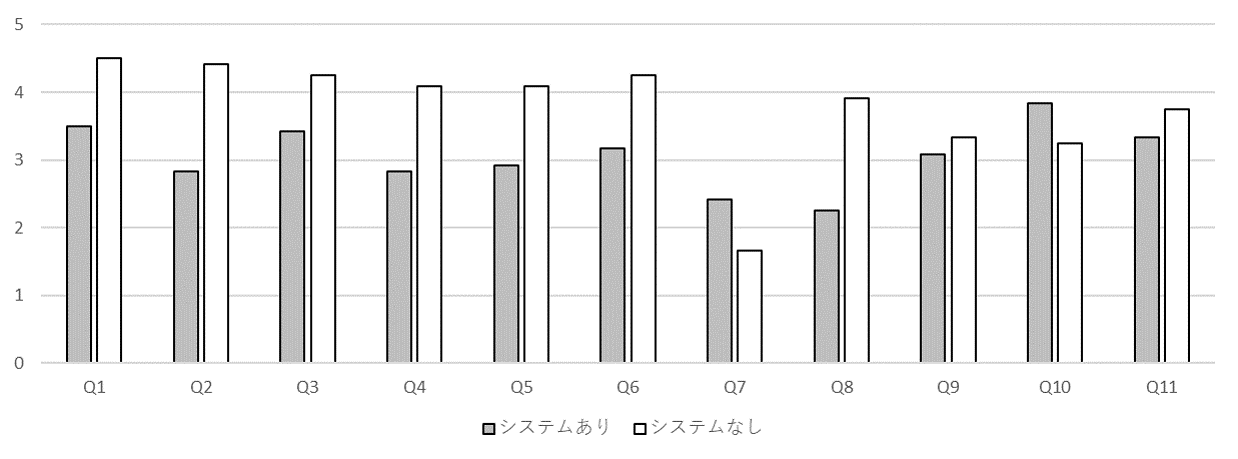
\includegraphics[width=150mm]{images/jikken1_situmonsi.png}
\caption{各設問への回答の平均値}
\label{fig:jikken1_kaito}
\end{center}
\end{figure}
\end{comment}

\begin{figure}[htbp]
\begin{center}
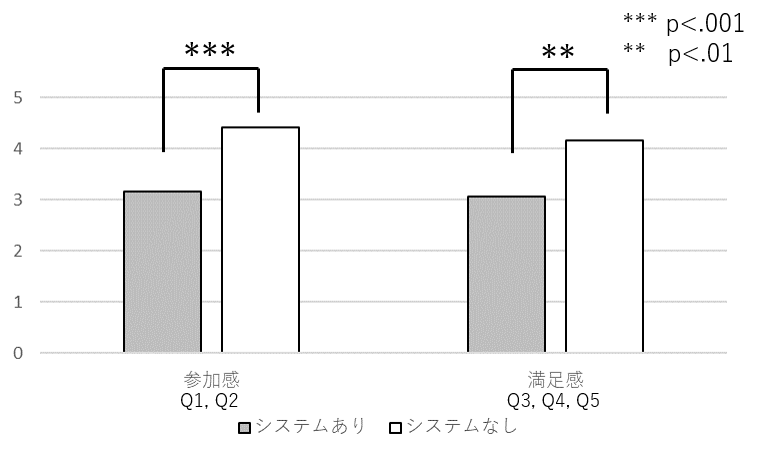
\includegraphics[width=100mm]{images/jikken1_manzoku.png}
\caption{参加感と満足感}
\label{fig:jikken1_sat}
\end{center}
\end{figure}

\begin{figure}[htbp]
\begin{center}
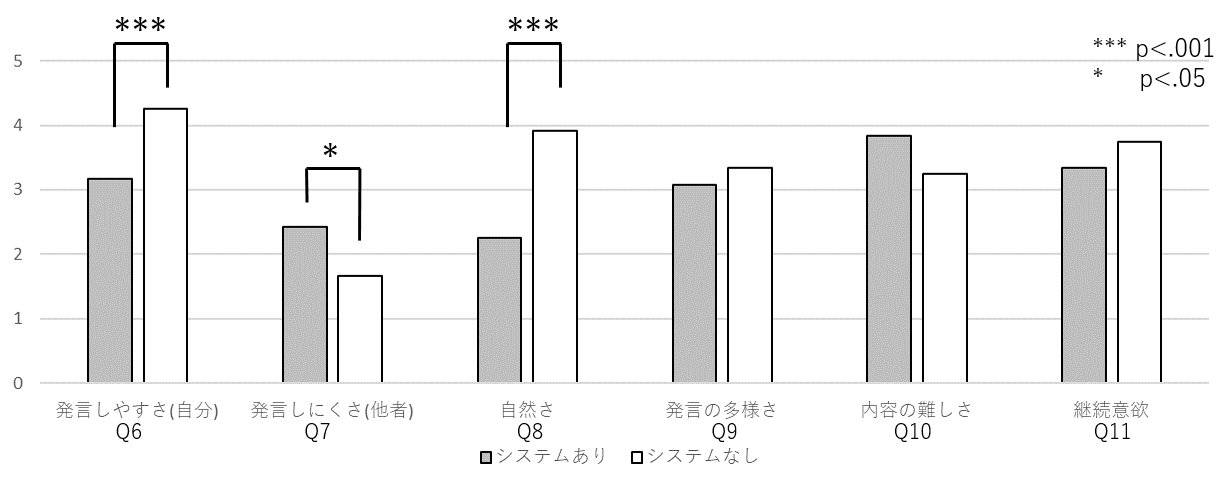
\includegraphics[width=150mm]{images/jikken1_kobetu}
\caption{個別の回答(Q6~Q11)}
\label{fig:jikken1_kobetu}
\end{center}
\end{figure}



\section{考察}
開発した議論システムRMSBD-1は十分な参加感および満足感をもたらすものではないことがわかった。また特に、実験参加者はシステムを使用した議論を自然ではないと評価していた。
システムを使用した議論中の操作履歴を分析したところ、各グループの発話回数およびインタフェース上の「更新」ボタンを押した回数は表\ref{tab:jikken1_log}のようになった。この表より、一度発話するごとに、参加者は何度も更新ボタンを押して別の選択肢を取得していたことがわかる。その結果、議論のペースが遅くなり、進行が不自然になったと考えられる。さらに、発話のない時間が続いたことは、参加感および満足感を低下させたと考えられる。

% Please add the following required packages to your document preamble:
% \usepackage{booktabs}
\begin{table}[]
\centering
\caption{グループごとの発話回数と更新ボタン押下回数}
\label{tab:jikken1_log}
\begin{tabular}{@{}llll@{}}
\toprule
\multicolumn{1}{c}{} & テーマ  & 発話回数 & 更新ボタン押下回数 \\ \midrule
グループ1                & 愛    & 36   & 650       \\
グループ2                & 愛    & 57   & 433       \\
グループ3                & 働くこと & 50   & 431       \\
グループ4                & 働くこと & 41   & 533       \\ \bottomrule
\end{tabular}
\end{table}


一方で、システムを使用した議論は、口頭での議論に比べ有意に低い参加感および満足感しかもたらさなかったが、議論の継続意欲や、意見の多様性の面では口頭での議論との遜色はなかった。


以上より、議論のペースを自然な速さにすることができれば、システムを使用した議論は、その後を促進するための導入として機能する可能性があると考えた。次章では、この点を踏まえて行ったシステムの再設計と、評価実験について報告する。





\chapter{議論支援システムの開発と評価実験2}

\section{システムの変更点}

\section{実験}

\subsection{検証項目}

\subsection{実験結果}

\section{考察}



\chapter{議論支援システムの開発と実証実験3}
%memo 三つ目のシステムは対立構造を作ることを目的に開発


\section{実験1、実験2で明らかになった問題点の整理}

\section{システムの設計}
\label{sec:システム3}
\section{議論シナリオの構成}

\section{仮説}

\section{実験}
\subsection{実験参加者}
大学生64名(男性32名、女性32名、平均年齢XX歳($SD=XX$))が4名1組で実験に参加した。参加者は(初対面かどうか)
\subsection{実験課題}
実験において、被験者は指定されたテーマについて議論を行うように指示された。テーマには、実際の哲学カフェのテーマを参考にし、「共感」と「死」選択した。[テーマを正当化する説明]


実験参加者は、同じ組のメンバと、異なるテーマについて2回議論を行う。それぞれの議論において、実験参加者は、議論を通してグループとしての結論を出すことを求められる。また、実験参加者は、議論開始時に主張する意見を表\ref{tab:始めの意見}に示したものから指定される。各テーマにおいて、それぞれの主張はランダムに2人ずつに対して与えられる。

\begin{table}[]
\caption{議論開始時に与えられた主張}
\centering
\begin{tabular}{@{}ll@{}}
\toprule
テーマ & \multicolumn{1}{c}{主張} \\ \midrule
死    & 死に際は美しい                \\
     & 死に際は醜いものだ              \\
共感   & 共感によって人は馬鹿になる          \\
     & 共感は人を成長させる             \\ \bottomrule
\end{tabular}
\label{tab:始めの意見}
\end{table}




\subsection{実験条件}
実験条件は、システムあり条件とシステムなし条件の2条件の被験者内計画であった。実験参加者グループは、表\ref{tab:順序}に示すいずれかの順序で議論を行った。それぞれの順序はカウンターバランスを取った。

\begin{table}[]
\caption{実験順序の組み合わせ}
\centering
\label{tab:順序}
\begin{tabular}{@{}lll@{}}
\toprule
  & \multicolumn{1}{c}{1回目の議論} & \multicolumn{1}{c}{2回目の議論} \\ \midrule
1 & 死(システムあり)                  & 共感(システムなし)                 \\
2 & 死(システムなし)                  & 共感(システムあり)                 \\
3 & 共感(システムあり)                 & 死(システムなし)                  \\
4 & 共感(システムなし)                 & 死(システムあり)                  \\ \bottomrule
\end{tabular}
\end{table}


\subsection{実験手続き}
実験参加者は、実験室に到着次第待合室で実験の説明を受けた後、実験室に設置された円形のテーブルに着席するように指示された。その後、全員の自己紹介を4分間で行った。このとき、実験者は「今回の実験では皆さんに議論をしていただきます。それに先立って、自己紹介をしていただきます。今から4分間で、全員が自己紹介をしてください。始まりはベルで指示するので、ベルが鳴ったらどなたからでもいいので自己紹介を始めてください。終了もベルで知らせますので、鳴ったら話すのを止めてください」と指示した。


自己紹介終了後、実験参加者は再度待合室に戻され、個別に質問紙(議論前1)に回答するように指示された。全員の記入が終わったことを確認したのち、実験者は議論後に記入させる質問紙(議論後1)の質問項目を印刷した紙を配布し、各項目の文言を確認させた。
また、システムあり条件を先に行うグループ(表\ref{tab:順序}の1と3)に対しては、システムの操作方法が印刷された紙を配布した。

各項目の文言に理解できないものが無いか確認後、再度実験室のテーブルに着席させた。その後、1回目の議論のテーマをグループ全員に口頭で伝えた。
その後、議論を行う前に議論開始時の立場を決めるための作業を行う旨を伝え、議論前準備の内容を教示した。議論前準備を始める前に、議論開始時に与えられる立場の選択肢を提示し、それが自分の意見とどのくらい近いかを回答させた(質問紙(議論前2))。その後、実験参加者に、個別に議論前準備として、システムあり条件では議論システムに文章を入力させ(システムへの入力項目は\ref{sec:システム3}を参照)、システムなし条件では、配布したワークシートの空欄を埋めさせた。ワークシートの項目と、システムへの入力の対応は図\ref{fig:対応表}に示した。

\begin{figure}[htbp]
\begin{center}
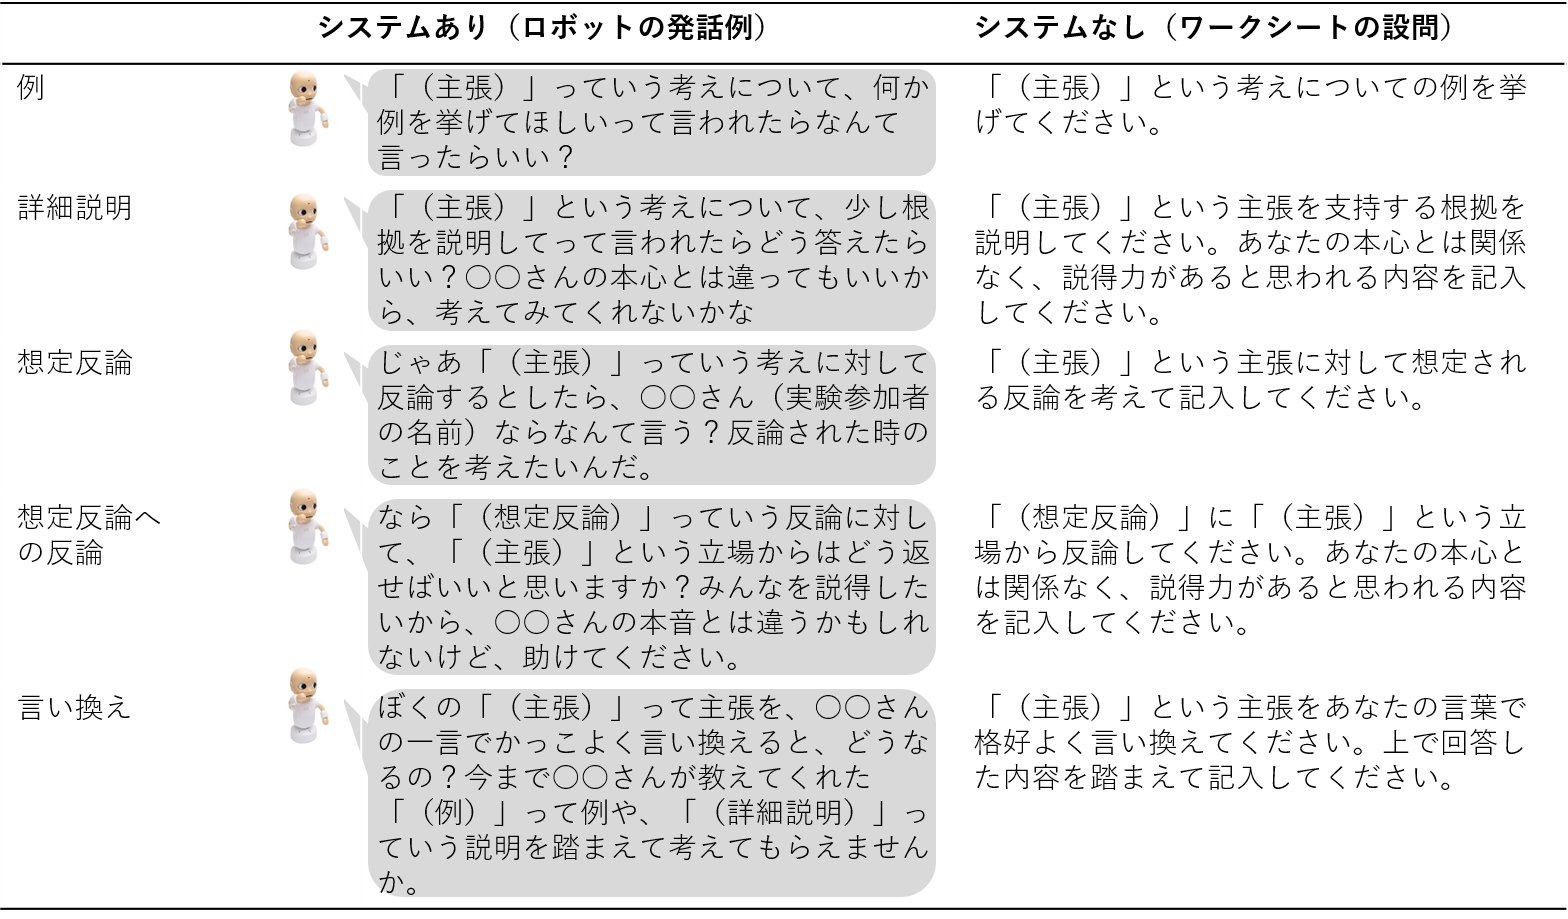
\includegraphics[width=150mm]{images/ワークとシステムの対応.png}
\caption{配布したワークシートの設問とロボットの発話の対応}
\label{fig:対応表}
\end{center}
\end{figure}

議論前準備を始めさせるにあたって行った教示内容を以下に示す。\\

\textbf{議論前準備の教示(システムあり条件)}
\begin{quote}
「(テーマ)」についての議論を行う前に、議論開始時点での立場を決めるために、皆さんのそばにいるロボットと相談していただきます。相談中は、手元のノートパソコンで選択肢を選ぶか、文章を入力していただきます。項目は全部で5つあります。制限時間は10分です。急がなくても記入できる分量になっていますので、焦らず入力してください。残り時間が3分になったら、一度お知らせします。
\end{quote}

\textbf{議論前準備の教示(システムなし条件)}
\begin{quote}
「(テーマ)」についての議論を行う前に、議論開始時点での立場を決めるために、今から配布するワークシートの空欄を埋めていただきます。記入の際は、選択肢に印をつけるか、文章を記入していただきます。項目は全部で5つあります。制限時間は10分です。急がなくても記入できる分量になっていますので、焦らず記入してください。残り時間が3分になったら、一度お知らせします。
\end{quote}


議論前準備を終えたのち、グループに議論を始めさせた。この際に行った教示内容を以下に記す。\\
\textbf{議論開始時の教示(システムあり条件)}
\begin{quote}
これからおよそ20分間、「(テーマ)」についてロボットと一緒に議論していただきます。まず、ロボット達が議論を切り出します。皆さんはその流れに従って議論に参加してください。この時、皆さんで結論を出すように努めて議論してください。結論の形式はどのようなものでも構いません。\footnote{ここの文言が思いつかない。二者択一しかダメだと解釈されないようにしたい}
残り時間が2分になったところで、結論を出すようにロボットが残り時間を伝えます。議論終了後には、個別に結論を記述していただきます。\footnote{結論を一人ずつ言わせる意味が分からなくなったので、筆記でもいい気がします}%一人一人結論を答えていただきます。
\end{quote}

\textbf{議論開始時の教示(システムなし条件)}
\begin{quote}
これからおよそ20分間、「(テーマ)」について皆さんで議論していただきます。まず、先ほど埋めたフォームに書かれた立場からの主張を行い、議論を開始してください。その後、皆さんで結論を出すように努めて議論してください。結論の形式はどのようなものでも構いません。残り時間が2分になったところで、結論を出すように実験者が残り時間を伝えます。議論終了後には、個別に結論を記述していただきます。%一人一人結論を答えていただきます。
\end{quote}



議論終了後には、机に着席したまま、各々の結論を5分間で白紙に記入させた。

%には、実験者がタイマーで時間を測り、1人1分以内で全参加者に議論の結論を述べさせた。
%その後
、机に着席したまま質問紙(議論後1)に回答させた。その後、1回目と同様の手続きを行い、2回目の議論を行った。2回目の議論の後には、2回の議論を比較するための質問紙(議論後2)に回答させた。


1回の議論の時間は22分と設定した。実験全体の所要時間は、およそ100分であった。以上の手続きをまとめると、表\ref{tab:進行3}になる。


\begin{figure}[htbp]
\begin{center}
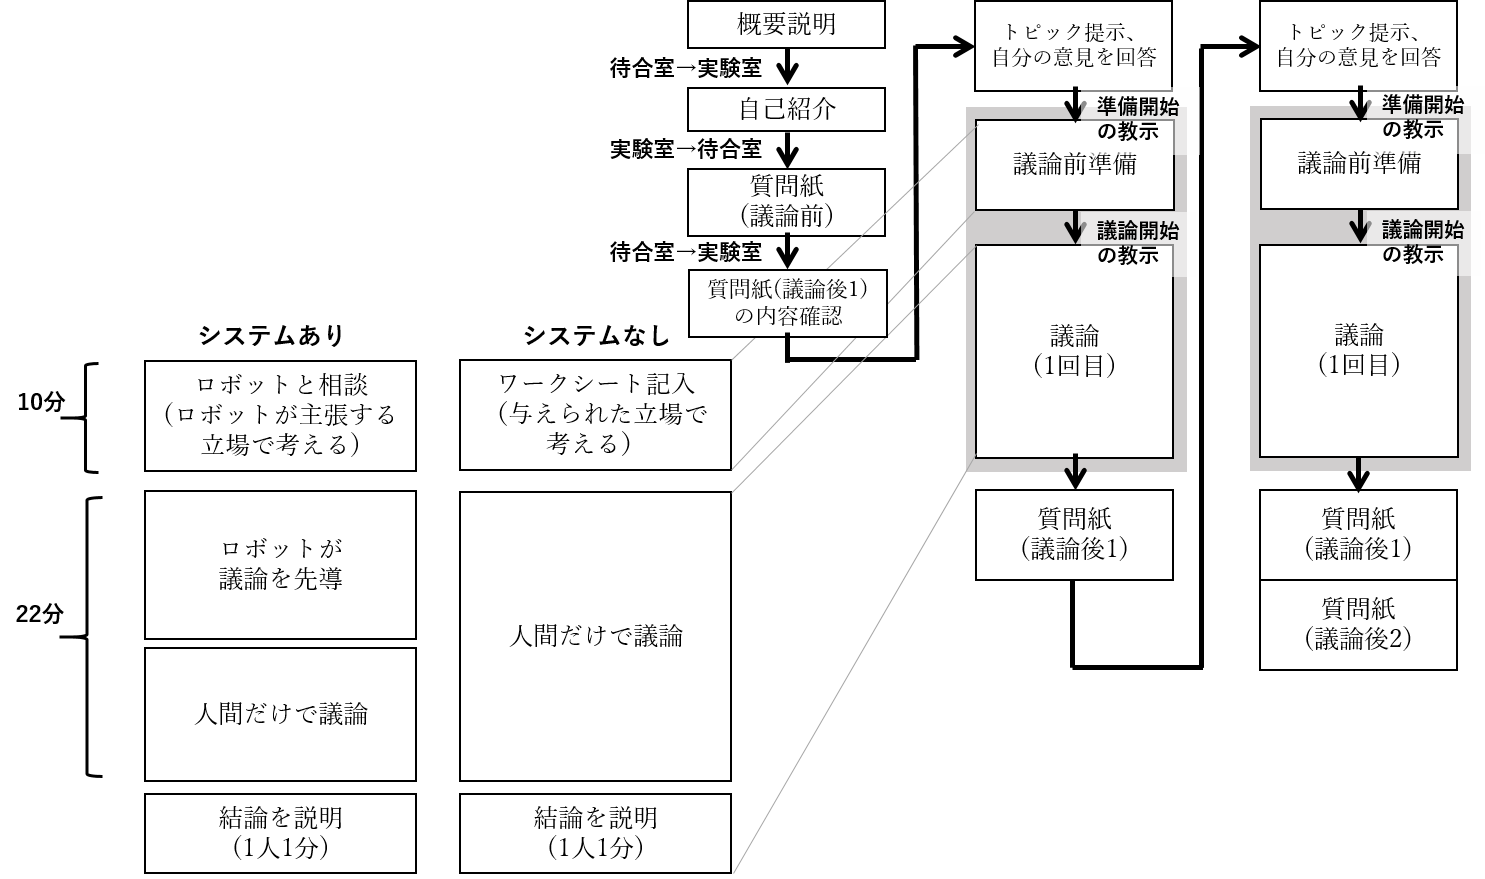
\includegraphics[width=150mm]{images/実験手続き.png}
\caption{実験手続き}
\label{fig:進行3}
\end{center}
\end{figure}


\subsection{測定指標}
%実験で使用した質問紙の項目を示す。
\subsubsection*{質問紙(議論前1)}
グループ内の親密さを測定するために、Inclusion of Other in Self” (IOS) scaleを使用した。この尺度では、他者との心理的な距離を視覚的に評価させる。
%ここでちゃんと説明する!!!!



また、議論における結論導出プロセスに影響を及ぼすことが知られている[引用(平山, 2004)]批判的思考力を、先行研究で用いたられた
「批判的思考態度尺度」を用いて、五件法(「1=あてはまらない」、「5=あてはまる」)議論前に測定した。ただし、(*)印がついた項目は反転項目である。質問項目には、因子負荷量が高い以下の11項目を使用した。表\ref{tab:hihanteki3}に示したこれらの項目は、先行研究で見出された全ての因子をカバーしている。
\begin{table}[H]
\caption{批判的思考態度尺度{[}引用{]}から抽出した質問項目}
\centering
\label{tab:hihanteki3}
\begin{tabular}{@{}ll@{}}
\toprule
\multicolumn{1}{c}{} & \multicolumn{1}{c}{質問項目} \\ \midrule
思考への自信               & 複雑な問題について順序だてて考えることが得意だ  \\
                     & 考えをまとめることが得意だ            \\
                     & 物事を正確に考えることに自信がある        \\
                     & 誰もが納得できるような説明をすることができる   \\
探求心                  & いろいろな考え方の人と接して多くのことを学びたい \\
                     & 生涯にわたり新しいことを学び続けたいと思う    \\
                     & 新しいものにチャレンジするのが好きである     \\
                     & さまざまな文化について学びたいと思う       \\
客観性                  & いつも偏りのない判断をしようとする        \\
                     & 物事を見るときに自分の立場からしか見ない(*)     \\
証拠の重視                & 結論をくだす場合には、確たる証拠の有無にこだわる \\ \bottomrule
\end{tabular}
\end{table}



さらに、表\ref{tab:daibo3}に示した6項目を用いて、コミュニケーション・スキルを測定した(かなり得意、得意、やや得意、ふつう、やや苦手、苦手、かなり苦手、の七件法)。これらは、[引用(藤本, 2007]で整理されたものである。
% Please add the following required packages to your document preamble:
% \usepackage{booktabs}
\begin{table}[H]
\caption{コミュニケーション・スキル尺度 ENDCORE(簡易版)[引用]}
\label{tab:daibo3}
\centering
\begin{tabular}{@{}ll@{}}
\toprule
\multicolumn{1}{c}{} & \multicolumn{1}{c}{質問項目}     \\ \midrule
自己統制                 & 自分の感情や行動をうまくコントロールする         \\
表現力                  & 自分の考えや気持ちをうまく表現する            \\
読解力                  & 相手の伝えたい考えや気持ちを正しく読み取る        \\
自己主張                 & 自分の意見や立場を相手に受け入れてもらえるように主張する \\
他者受容                 & 相手を尊重して相手の意見や立場を理解する         \\
関係調整                 & 周囲の人間関係にはたらきかけ良好な状態に調整する     \\ \bottomrule
\end{tabular}
\end{table}


\subsubsection*{質問紙(議論前2)}
本実験では、「「ロボットへの助言者」という立場を与えることによって、自分の本心とは異なる意見であっても意欲や責任感を失わず、ある特定の立場を受け入れて主体的な主張を行うことができる」、という仮説を検証する必要がある。そこで、議論前に立場を与えるよりも先に、実験参加者の元の意見を取得する必要がある。よって、以下のような質問項目を作成した。ここで、議論前に与える2つの立場は、背反であることは自明ではない。また、どちらの立場にも同意している参加者と、どちらの立場にも同意していない参加者とでは、2つの立場に対して「中立的」であっても、議論に対する意欲や責任感の感じ方には相違があると考えられる。以上から、二者択一、あるいは左右に2つの意見を配置したデザインではなく、提示された立場と自らの意見との関係を個別に七件法(「1=全くそう思わない」、「7=とてもそう思う」)で回答させた(表\ref{tab:motonoiken})。
% Please add the following required packages to your document preamble:
% \usepackage{booktabs}
\begin{table}[H]
\caption{元の意見の聴取}
\centering
\label{tab:motonoiken}
\begin{tabular}{@{}ll@{}}
\toprule
\multicolumn{1}{c}{テーマ} & \multicolumn{1}{c}{質問項目}  \\ \midrule
死                        & あなたは「死に際は美しい」と思いますか       \\
                         & あなたは「死に際は醜い」と思いますか        \\
共感                       & あなたは「共感によって人は馬鹿になる」と思いますか \\
                         & あなたは「共感は人を成長させる」と思いますか    \\ \bottomrule
\end{tabular}
\end{table}
\begin{comment}
\begin{itemize}
\setlength{\parskip}{-0.1cm} % 段落間
  \setlength{\itemsep}{-0.1cm} % 項目間
\item あなたの意見はどちらに近いですか(「死に際は美しい」、「死に際は醜い」の二択)
\end{itemize}
もしくは、
\begin{itemize}
\setlength{\parskip}{-0.1cm} % 段落間
  \setlength{\itemsep}{-0.1cm} % 項目間
\item あなたの意見はどちらに近いですか(「共感によって人は馬鹿になる」、「共感は人を成長させる」の二択)
\end{itemize}
\end{comment}

%\begin{itemize}
%\setlength{\parskip}{-0.1cm} % 段落間
 % \setlength{\itemsep}{-0.1cm} % 項目間
%\item あなたは「死に際は美しい」と思いますか
%\item あなたは「死に際は醜い」と思いますか
%\end{itemize}

%もしくは、

%\begin{itemize}
%\setlength{\parskip}{-0.1cm} % 段落間
  %\setlength{\itemsep}{-0.1cm} % 項目間
%\item あなたは「共感によって人は馬鹿になる」と思いますか
%\item あなたは「共感は人を成長させる」と思いますか
%\end{itemize}


\subsubsection*{質問紙(議論後1)}
実験参加者は、システムあり条件とシステムなし条件では、前者では「ロボットへの助言者」として、後者では「指定された立場で発言する人」として議論に参加する。
本実験では、前者の方が、自分の本来の意見とは違う立場であっても意欲と責任感を感じやすいという仮説を立てている。

また、「ロボットへの助言者」としての役割で、意見対立のある議論に参加することが、満足感や参加感に与える影響を調査することも本実験の目的である。以上を踏まえ、表\ref{tab:indev}に示すように、議論に対する総合的な主観評価として、以下の質問項目を七件法(「1=全くそう思わない」、「7=とてもそう思う」)で回答させた。
%仮説検証はこの項目で、それ以外の分析はおまけ


% Please add the following required packages to your document preamble:
% \usepackage{booktabs}
\begin{table}[H]
\caption{議論に対する総合的な主観評価}
\centering
\label{tab:indev}
\begin{tabular}{@{}ll@{}}
\toprule
\multicolumn{1}{c}{} & \multicolumn{1}{c}{質問項目} \\ \midrule
意欲と責任                & 議論中に、あなたは指定された役割を果たそうとした \\
                     & 指定された役割を果たすのは難しかった       \\
満足感                  & 先ほどの議論は楽しかった             \\
                     & 先ほどの議論に満足している            \\
                     & 先ほどの議論は深まった              \\
参加感                  & 議論に参加したという感覚が強くある        \\
                     & グループの結論に自分は貢献できた         \\ \bottomrule
\end{tabular}
\end{table}


議論中の葛藤を測定する尺度として、[引用(村山ら2013)]を参考に、[引用(Jehn et al., 1994)]を翻訳した
9項目に対し、
七件法(「1=全くなかった」、「7=かなりあった」)で回答させた。表\ref{tab:conflict}に示したこの尺度は広く用いられており、[引用(Pearson et al., 2002)]でも妥当性が確認されている。分析の際は、下位尺度の平均値を用いた。

% Please add the following required packages to your document preamble:
% \usepackage{booktabs}
\begin{table}[H]
\centering
\caption{集団内葛藤の尺度{[}引用{]}}
\label{tab:conflict}
\begin{tabular}{@{}ll@{}}
\toprule
\multicolumn{1}{c}{} & \multicolumn{1}{c}{質問項目}                                                                     \\ \midrule
関係葛藤                 & 議論をしたグループの人々の間では、不和はどの程度ありましたか                                                               \\
                     & 議論をしたグループの人々の間では、性格的な衝突はどの程度ありましたか                                                           \\
                     & 議論をしたグループの人々の間では、緊張はどの程度ありましたか                                                               \\
                     & 議論をしたグループの人々の間では、感情的な対立はどの程度ありましたか                                                           \\
                     & 議論をしたグループの人々の間では、腹立たしい気持ちはどの程度ありましたか                                                         \\
課題葛藤                 & 議論をしたグループの人々の間では意見の対立はどの程度ありましたか                                                                  \\
                     & 異なる意見の間での対立はどのくらい多くありましたか\\
                     & \begin{tabular}[c]{@{}l@{}}\vspace{-0.15cm}議論をしたグループの人々の間では、結論に関わる考えの相違はどのくらい\\ 多くありましたか\end{tabular} \\
                     & 議論を行ったグループの人々の間では、意見の相違はどのくらい多くありましたか                                                             \\ \bottomrule
\end{tabular}
\end{table}


議論中に出た意見の間での葛藤を測定する尺度として、に表\ref{tab:conflict2}示した質問項目を用いた。集団内葛藤の尺度を参考に、程度と頻度を尋ねる設問を設定した。
\begin{table}[H]
\centering
\caption{議論中に出た意見間での葛藤の尺度{[}引用{]}}
\label{tab:conflict2}
\begin{tabular}{@{}ll@{}}
\toprule
\multicolumn{1}{c}{質問項目}              \\ \midrule
議論(約20分全体を通して)で出た意見は、どの程度対立していましたか                    \\
議論(約20分全体を通して)で出た意見は、どのくらい頻繁に対立していましたか \\ \bottomrule
\end{tabular}
\end{table}



「ロボットへの助言者」として議論に参加していることが、集団内葛藤に対する対処行動として統合的対処行動を増加させるのかを調査することも、本研究の目的である。
議論中に行った葛藤対処行動を測定する尺度として、[引用(村山ら2013)]を参考に、葛藤に対する5種類の対処行動を測定する尺度(The Dutch Test for Conflict Handling; Van de Vliert (1997))からそれぞれ因子負荷量の高い上位2項目ずつを用いた。質問項目は表\ref{tab:conflict_deal}に示した。
先行研究に倣い、「意見がまとまらなかったり対立が起こったとき、あなたは以下の行動をどの程度とりましたか」という教示の下で、七件法(「1=全くそうしなかった」、「7=かなりそうした」)で回答させた。
下位尺度は合算し、平均値を分析対象とした。


% Please add the following required packages to your document preamble:
% \usepackage{booktabs}
\begin{table}[H]
\caption{葛藤対処行動({[}引用{]}から抽出)}
\centering
\label{tab:conflict_deal}
\begin{tabular}{@{}ll@{}}
\toprule
\multicolumn{1}{c}{} & \multicolumn{1}{c}{質問項目}             \\ \midrule
譲歩                   & 他のメンバーの目的や興味に合わせた                    \\
                     & 他のメンバーに同意しようとした                      \\
妥協                   & お互いが少しずつ歩み寄ることにこだわった                 \\
                     & 妥協的な解決策を見つける必要があると強調した               \\
主張                   & 自分の主張を推し進めた                          \\
                     & 自分にとって良い結果が得られるように努めた                \\
統合                   & 自分と他のメンバーの興味ができる限り反映されるような結論を見出そうとした \\
                     & 最適な解決策を見つけるために意見を吟味した                \\
回避                   & 意見の相違をできるだけ避けた                       \\
                     & 他のメンバーと対立することを避けようとした                \\ \bottomrule
\end{tabular}
\end{table}




また、「ロボットへの助言者」として議論に参加することが、議論の質にどのような影響を与えるのかを探索的に検討するため、
統合的対処行動の達成度評価、議論における自己開示度、の評価を七件法(「1=全くそう思わない」、「7=とてもそう思う」)で回答させ、主観的議論時間を回答させた(表\ref{tab:search})。

\begin{table}[H]
\centering
\caption{「ロボットへの助言者」として議論参加する効果の探索的調査}
\label{tab:search}
\begin{tabular}{@{}ll@{}}
\toprule
\multicolumn{1}{c}{} & \multicolumn{1}{c}{質問項目}                                                        \\ \midrule
統合的対処行動の達成度          & あなたは異なる意見の統合にどのくらい貢献出来ましたか                                                      \\
                     & \begin{tabular}[c]{@{}l@{}}\vspace{-0.15cm}グループで出した結論には、議論中に出た異なる意見が多く\\ 反映されていた\end{tabular}   \\
議論における自己開示           & 自分の本音を他の人々と共有できた                                                                \\
                     & グループの人々の率直な意見を聞くことができた                                                          \\ \bottomrule
\end{tabular}
\end{table}




\subsubsection*{質問紙(議論後2)}
システムあり条件の議論とシステムなし条件の議論の好感度を比較するために、表\ref{tab:koukando}に示す質問項目を二者択一(「ロボットがいた議論」または「人だけの議論」)で回答させた。

% Please add the following required packages to your document preamble:
% \usepackage{booktabs}
\begin{table}[H]
\caption{議論に対する好感度の比較}
\centering
\label{tab:koukando}
\begin{tabular}{@{}l@{}}
\toprule
\multicolumn{1}{c}{質問項目}              \\ \midrule
議論はどちらが楽しかったですか                       \\
開始直後の自己紹介から結論までの議論の進行は、どちらがやりやすかったですか \\
どちらの議論でより言いたいことが言えましたか                \\
どちらの議論が他の人の意見を聞きやすかったですか   	\\          
もう一回今回のグループで議論するとしたらどちらの条件で議論したいですか \\ \bottomrule
\end{tabular}
\end{table}



システムあり条件の議論が、どのような議題に対し有効だと実験参加者が感じたのかを検討するため、
表\ref{tab:cond}に示した質問項目に、二者択一(「ロボットがいた議論」または「人だけの議論」)で回答させた。

% Please add the following required packages to your document preamble:
% \usepackage{booktabs}
\begin{table}[]
\caption{どのような議論なら今回のシステムが欲しいか}
\label{tab:cond}
\begin{tabular}{@{}l@{}}
\toprule
\multicolumn{1}{c}{質問項目}                                                                 \\ \midrule
	以下の話題はどちらの条件で議論したいですか                                                                    \\
	\hspace{0.5cm}朝食はパンかご飯か                                                                                \\
	\hspace{0.5cm}日本は捕鯨をやめるべきか                                                                             \\
	\hspace{0.5cm}死刑制度は存続すべきか                                                                              \\
	\hspace{0.5cm}愛とは何か                                                                                    \\	
	\hspace{0.5cm}絶対的な悪は存在するか                                                                              \\
\begin{tabular}[c]{@{}l@{}}今日話したテーマに限らず、以下の状況での様々な議論で、どちらの条件で議論したいですか\\\end{tabular} \\
	\hspace{0.5cm}講義中のグループワークでの議論                                                                          \\
	\hspace{0.5cm}サークルや部活動での決めごとに関する議論                                                                     \\	
	\hspace{0.5cm}友達との議論                                                                                   \\
	\hspace{0.5cm}嫌いな人との議論                                                                                 \\
	\hspace{0.5cm}家族との議論                                                                                   \\
	\hspace{0.5cm}初対面の人との議論                                                                                \\ \bottomrule
\end{tabular}
\end{table}




また、実験参加者が本実験で利用したシステムを再度使いたいという気持ちをどれだけ持ったかを測定するために、表\ref{tab:intention}の質問項目に自由記述で回答させた。
\begin{table}[H]
\caption{今回のシステムを使いたいか・どんな状況で使いたいか}
\centering
\label{tab:intention}
\begin{tabular}{@{}l@{}}
\toprule
\multicolumn{1}{c}{質問項目}              \\ \midrule
ロボットを使ったシステムをまた使ってみたいですか\\
ロボットを使ったシステムはいつ使ってみたい、あるいは使ってみたかったですか\\
ロボットを使ったシステムは誰と使ってみたいですか \\ \bottomrule
\end{tabular}
\end{table}

\subsection{実験結果}

\section{考察}




\chapter{結論}

\chapter*{謝辞}
\addcontentsline{toc}{chapter}{謝辞}%目次に表示するためのやつ
謝辞

%%%%%%%%%%%%%%%%%%%%%%%%%%%
%参考文献
%%%%%%%%%%%%%%%%%%%%%%%%%%%
\bibliographystyle{junsrt}%参考文献を番号順に
\bibliography{bunken} %bunken.bibを参照している
\addcontentsline{toc}{chapter}{\bibname}%目次に表示するためのやつ

\end{document}